\clearpage
\VerdierPhysicalPageAnchor{0082}%
\VerdierSemanticAnchor{ch1-3}
\section{特异三角}

\VerdierSemanticAnchor{ch1-3-1}
\subsection{态射的映射锥}

\VerdierSemanticAnchor{ch1-3-1-1}
\noindent\textbf{3.1.1.}\quad
\VerdierSemanticAnchor{ch1-3-1-1-tr1-category}
设 $C$ 是加法范畴。以 $\operatorname{tr}_1(C)$ 表示如下范畴：

\VerdierSemanticAnchor{ch1-3-1-1-objects}
\noindent--\quad $\operatorname{tr}_1(C)$ 的对象是 $C$ 中对象的复形之间的
（零次）态射 $X\xrightarrow{f}Y$。

\VerdierSemanticAnchor{ch1-3-1-1-morphisms}
\noindent--\quad 设 $X\xrightarrow{f}Y$ 和 $X'\xrightarrow{f'}Y'$ 是
$\operatorname{tr}_1(C)$ 的两个对象。从 $X\xrightarrow{f}Y$ 到
$X'\xrightarrow{f'}Y'$ 的一个态射是三元组 $(g,h,a)$，其中
$g\colon X\longrightarrow X'$ 与 $h\colon Y\longrightarrow Y'$ 是零次复形态射，
而
\VerdierSemanticAnchor{ch1-3-1-1-homotopy-data}
$a\colon f'g\rightsquigarrow hf$ 是连接 $f'g$ 与 $hf$ 的同伦。

\VerdierSemanticAnchor{ch1-3-1-1-composition}
\noindent--\quad 设
\begin{equation*}
  \begin{aligned}
    (g,h,a)\colon (X\xrightarrow{f}Y)
      &\longrightarrow (X'\xrightarrow{f'}Y'),\\
    (g',h',a')\colon (X'\xrightarrow{f'}Y')
      &\longrightarrow (X''\xrightarrow{f''}Y'')
  \end{aligned}
\end{equation*}
是 $\operatorname{tr}_1(C)$ 的两个态射。其复合态射
\begin{equation*}
  (g'',h'',a'')\colon
  (X\xrightarrow{f}Y)\longrightarrow(X''\xrightarrow{f''}Y'')
\end{equation*}
由下列等式定义：

\VerdierSemanticAnchor{ch1-3-1-1-eq1}
\begin{equation}
  \begin{aligned}
    g''&=g'g,\\
    h''&=h'h,\\
    a''&=a'\star g+h'\star a.
  \end{aligned}
  \tag{3.1.1.1}
\end{equation}

\VerdierSemanticAnchor{ch1-3-1-1-category-verification}
立即可验证，这样确实定义了一个范畴。
\VerdierSemanticAnchor{ch1-3-1-1-diagram-representation}
我们通常用下图表示 $\operatorname{tr}_1(C)$ 的态射
$(g,h,a)\colon(X\xrightarrow{f}Y)\longrightarrow(X'\xrightarrow{f'}Y')$：

\VerdierSemanticAnchor{ch1-3-1-1-eq2}
\begin{equation}
  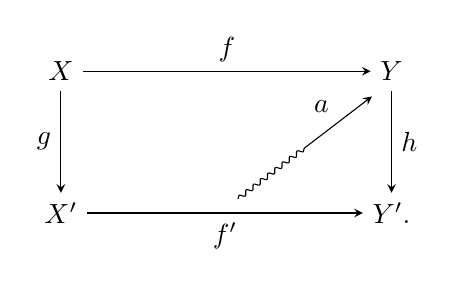
\begin{tikzpicture}[>=stealth,baseline=(current bounding box.center)]
    \node (X)  at (0,1.8) {$X$};
    \node (Y)  at (4.2,1.8) {$Y$};
    \node (Xp) at (0,0) {$X'$};
    \node (Yp) at (4.2,0) {$Y'\mathpunct{.}$};
    \draw[->] (X) -- node[above] {$f$} (Y);
    \draw[->] (X) -- node[left] {$g$} (Xp);
    \draw[->] (Y) -- node[right] {$h$} (Yp);
    \draw[->] (Xp) -- node[below] {$f'$} (Yp);
    \draw[decorate,decoration={snake,amplitude=0.8pt,segment length=3.3pt}]
      (2.25,0.18) -- (3.10,0.83);
    \draw[->] (3.10,0.83) -- node[above left] {$a$} (3.95,1.48);
  \end{tikzpicture}
  \tag{3.1.1.2}
\end{equation}
